% =====================================================================
%  Informe: Planteamiento del problema
%  Caso XM - UNAL: precio de bolsa y garantía de las exportaciones a Ecuador
%  Compilar con pdfLaTeX (Overleaf: Menu > Compiler > pdfLaTeX)
% =====================================================================
\documentclass[11pt,letterpaper]{article}

% ---------- Idioma y tipografía ----------
\usepackage[utf8]{inputenc}
\usepackage[T1]{fontenc}
\usepackage[spanish,es-noshorthands,es-tabla,es-nodecimaldot]{babel}
\usepackage{lmodern}
\usepackage{microtype}

% ---------- Página ----------
\usepackage[margin=2.5cm]{geometry}
\usepackage{setspace}
\onehalfspacing
\setlength{\parskip}{4pt}
\usepackage{fancyhdr}
\pagestyle{fancy}
\fancyhf{}
\lhead{\small\itshape Caso XM--UNAL}
\rhead{\small\itshape Planteamiento del problema}
\cfoot{\small\thepage}
\renewcommand{\headrulewidth}{0.4pt}
\setlength{\headheight}{14pt}

% ---------- Matemáticas, tablas y figuras ----------
\usepackage{amsmath,amssymb}
\usepackage{booktabs}
\usepackage{tabularx}
\usepackage{array}
\usepackage{graphicx}
\usepackage{float}
\usepackage{caption}
\captionsetup{font=small,labelfont=bf,labelsep=period}
\usepackage{enumitem}
\setlist{itemsep=2pt,topsep=4pt}

% ---------- Diagramas ----------
\usepackage{xcolor}
\definecolor{azul}{HTML}{1F3A5F}
\definecolor{gris}{HTML}{5F6B7A}
\definecolor{claro}{HTML}{EEF2F7}
\usepackage{tikz}
\usetikzlibrary{arrows.meta,positioning,babel}
\usepackage{pgfplots}
\pgfplotsset{compat=1.18}
\pgfkeys{/pgf/number format/.cd,use comma,1000 sep={.}}

\usepackage[hidelinks]{hyperref}

\newcommand{\cop}{\,COP/kWh}
\newcolumntype{L}{>{\raggedright\arraybackslash}X}

% =====================================================================
\begin{document}

% ---------- Portada ----------
\begin{titlepage}
  \centering
  \vspace*{1cm}
  {\large\scshape Universidad Nacional de Colombia\par}
  \vspace{0.2cm}
  {\scshape Caso de estudio XM -- UNAL\par}
  \vspace{3cm}
  {\LARGE\bfseries Planteamiento del problema\par}
  \vspace{0.6cm}
  {\Large Incertidumbre del precio de bolsa en la fijación de\\[2pt]
  la garantía de las exportaciones de energía a Ecuador\par}
  \vspace{3cm}
  {\large Carlos Acevedo\par}
  \vfill
  {Bogotá, noviembre de 2026\par}
\end{titlepage}

% ---------- Índice ----------
\pagenumbering{roman}
\tableofcontents
\newpage

% ---------- Resumen ----------
\section*{Resumen}
\addcontentsline{toc}{section}{Resumen}
\noindent
Las exportaciones de energía de Colombia a Ecuador se liquidan con el
precio de bolsa del Mercado de Energía Mayorista, un valor que solo se
conoce después de transcurrida la semana. La garantía que respalda esas
operaciones, en cambio, debe constituirse antes. Este informe plantea el
problema que surge de ese desfase: el monto se compromete sin una
estimación del precio que sea verificable, que esté disponible a tiempo
y cuya probabilidad de quedarse corta sea conocida. A partir de los
datos públicos de XM entre 2010 y 2026 se describe la situación actual,
se dimensiona la brecha frente a la situación deseada, se distinguen los
hechos comprobados de los supuestos que aún dependen de XM, se analizan
las causas y se delimita el alcance. El informe cierra con la pregunta
de investigación, los objetivos y una síntesis del trabajo exploratorio
realizado, cuyos resultados ayudaron a precisar el propio problema. Entre
ellos, el más relevante es que la información disponible ---y por tanto
la calidad de cualquier estimación--- depende sobre todo del momento en
que se fije la garantía.

\medskip
\noindent\textbf{Palabras clave:} mercado eléctrico colombiano, precio de
bolsa, transacciones internacionales de electricidad, garantías,
incertidumbre, planteamiento del problema.

\newpage
\pagenumbering{arabic}

% =====================================================================
\section{Introducción}
% =====================================================================

En los mercados eléctricos, buena parte de las decisiones financieras se
toman antes de conocer el precio al que finalmente se liquidará la
energía. Colombia no es la excepción. El precio de bolsa del Mercado de
Energía Mayorista (MEM) se forma hora a hora y se consolida días
después, mientras que los compromisos que dependen de él ---como las
garantías que respaldan las exportaciones a Ecuador--- deben quedar
definidos con anticipación.

El caso XM--UNAL surgió como una propuesta concreta: construir un
pronóstico semanal del precio de bolsa. Sin embargo, una propuesta
formulada desde la herramienta corre el riesgo de resolver con precisión
un problema que no está bien definido. Por eso, antes de discutir
cualquier solución, este documento se detiene en el problema mismo:
quién lo padece, en qué consiste exactamente, qué evidencia lo respalda,
por qué ocurre y hasta dónde debe abordarse.

El informe se organiza así. La Sección~\ref{sec:contexto} presenta el
contexto del mercado y de los intercambios con Ecuador. La
Sección~\ref{sec:problema} describe el problema y la brecha entre la
situación actual y la deseada, y la Sección~\ref{sec:actores} identifica
a quienes la sufren. La Sección~\ref{sec:evidencia} reúne la evidencia
disponible, separando lo comprobado de lo supuesto, y la
Sección~\ref{sec:causas} analiza las causas. Las
Secciones~\ref{sec:alcance} y~\ref{sec:pregunta} delimitan el alcance y
formulan la pregunta de investigación y los objetivos. Finalmente, la
Sección~\ref{sec:avance} resume el trabajo exploratorio realizado y lo
que este enseñó sobre el problema.

% =====================================================================
\section{Contexto}
\label{sec:contexto}
% =====================================================================

\subsection{El precio de bolsa en Colombia}

El precio de bolsa resulta del cruce entre las ofertas de los
generadores y la demanda de cada hora. Como la mayor parte de la
capacidad instalada del país es hidráulica, el precio está ligado de
forma estrecha a la disponibilidad de agua. Cuando los embalses están
llenos y los aportes de los ríos son abundantes, la energía es barata;
en temporadas secas, y en particular bajo el fenómeno de El Niño, entran
en operación las plantas térmicas, más costosas, y el precio puede
multiplicarse en pocas semanas. Entre 2010 y 2026 el precio promedio
semanal osciló entre menos de 100 y más de 1.000\cop.

Para referirse al precio de una semana completa, este trabajo usa el
promedio de las 168 horas de lunes a domingo, ponderado por la demanda
de cada hora:
\begin{equation}
  P_s \;=\; \frac{\sum_{h\in s} P_h\,D_h}{\sum_{h\in s} D_h},
  \label{eq:precio}
\end{equation}
donde $P_h$ es el precio de bolsa y $D_h$ la demanda comercial en la
hora~$h$. De este modo las horas de mayor consumo pesan más, como ocurre
en la liquidación de la energía. Esta definición, sin embargo, es una
elección del proyecto que debe contrastarse con la regla de liquidación
de XM.

\subsection{Los intercambios con Ecuador}

Colombia y Ecuador están interconectados eléctricamente y comercian
energía a través de las Transacciones Internacionales de Electricidad
(TIE). Cuando Colombia exporta, la operación se liquida con precios que
solo se conocen una vez ocurrida la semana. Para cubrir el riesgo de que
la contraparte no pague, la transacción se respalda con una garantía o
un prepago que debe constituirse de antemano. En ese desfase
---comprometer hoy un monto que depende de un precio futuro--- se
origina el problema que estudia este informe.

\subsection{Cambios recientes en el entorno}

El año 2026 trajo cambios que no pueden ignorarse. Desde el 7 de
septiembre no hay exportaciones por TIE a Ecuador, tras la activación
del período de riesgo de desabastecimiento. La Resolución CREG 101~127
de 2026~\cite{creg2026} suspendió de forma transitoria el estatuto vigente desde 2014,
reguló las ofertas de las plantas hidráulicas mediante una curva y
estableció que los cargos de exportación consideren el mayor valor entre
el Precio de Bolsa TIE, el costo de la planta más cara y el costo
marginal del país importador. A su vez, la Resolución 40308 de 2026
habilitó contratos bilaterales entre agentes privados, en los cuales las
diferencias deben ser respaldadas y prepagadas por las partes.

Estos hechos no eliminan el problema, pero lo vuelven condicional:
obligan a precisar si la necesidad sigue vigente, qué precio interviene
realmente en la garantía y si la historia del mercado sigue siendo
representativa. La lectura normativa presentada aquí proviene de los
textos públicos y no constituye una interpretación oficial.

% =====================================================================
\section{Descripción del problema}
\label{sec:problema}
% =====================================================================

\subsection{Situación actual}

Hoy, la garantía que respalda las exportaciones de energía a Ecuador se
fija antes de conocer el precio de bolsa con el que se liquidará la
semana. No existe una estimación de ese precio que sea verificable, que
esté disponible en el momento de decidir y que indique cuánto puede
equivocarse. En consecuencia, no es posible saber con qué frecuencia el
monto comprometido resulta insuficiente ni cuánto capital se inmoviliza
de más.

A esto se suma una restricción de información. Los datos públicos del
mercado se publican con rezago: el precio y la demanda de un día suelen
estar disponibles unos tres días después. Quien decide al comienzo de
una semana, por tanto, no conoce todavía cómo cerró la anterior, que es
precisamente la información más útil para anticipar la siguiente.

\subsection{Situación deseada}

Lo deseable es que, al momento de fijar la garantía, se disponga de una
estimación del precio de la semana siguiente acompañada de un valor
superior cuya confiabilidad sea conocida; por ejemplo, un valor que el
precio real no supere en nueve de cada diez semanas. Ese valor permitiría
dimensionar la garantía con un nivel de riesgo explícito, medir
cuánto se inmoviliza de más y revisar después, con datos, si el criterio
funcionó.

\subsection{La brecha}

La distancia entre ambas situaciones puede describirse en tres
dimensiones medibles, resumidas en la Figura~\ref{fig:brecha}:

\begin{itemize}
  \item \textbf{Exactitud.} La referencia más simple disponible, suponer
        que la próxima semana costará lo mismo que la actual, se equivoca
        en promedio 66,6\cop{} entre 2018 y 2026, y 116,5\cop{} en los
        años de estrés hídrico de 2022 a 2024.
  \item \textbf{Confiabilidad.} No existe un valor superior del precio
        cuya frecuencia de cumplimiento se conozca, de modo que no es
        posible afirmar si una garantía es suficiente.
  \item \textbf{Oportunidad.} Debido al rezago de publicación, la semana
        de referencia solo queda completa hacia el miércoles, cuando la
        semana que se quiere anticipar ya lleva dos días en curso. Con la
        información pública, la ``semana de antelación'' que planteaba la
        propuesta inicial no existe. Además, no está definido en qué
        momento debe fijarse la garantía, y de ese momento depende qué
        información está disponible para decidir.
\end{itemize}

\begin{figure}[H]
\centering
\begin{tikzpicture}[
  bloque/.style={rectangle,draw=gris,line width=0.6pt,text width=4.1cm,
                 minimum height=3.3cm,align=left,font=\small,inner sep=6pt},
  flecha/.style={-{Stealth[length=3mm]},line width=0.8pt,gris}]
  \node[bloque] (a) {
    \textbf{Situación actual}\\[3pt]
    Garantía fijada sin una estimación verificable del precio.
    Se desconoce con qué frecuencia queda corta. Datos con unos tres
    días de rezago.};
  \node[bloque,fill=claro,right=0.9cm of a] (b) {
    \textbf{Brecha}\\[3pt]
    Sin medida de la confiabilidad del monto. Sin antelación real al
    decidir. Mayor error cuando el precio sube.};
  \node[bloque,right=0.9cm of b] (c) {
    \textbf{Situación deseada}\\[3pt]
    Estimación disponible al decidir, con un valor superior de
    cumplimiento conocido y un exceso de garantía acotado.};
  \draw[flecha] (a) -- (b);
  \draw[flecha] (b) -- (c);
\end{tikzpicture}
\caption{Brecha entre la situación actual y la deseada.}
\label{fig:brecha}
\end{figure}

\subsection{Enunciado del problema}

Con base en lo anterior, el problema puede enunciarse así:

\begin{quote}
\itshape
La garantía semanal de las exportaciones de energía a Ecuador se fija
sin una estimación del precio de bolsa de la semana siguiente que esté
disponible en el momento de decidir y cuya probabilidad de quedar por
debajo del precio real sea conocida. Esto expone al mercado a garantías
insuficientes en las semanas de alza y a capital inmovilizado de más en
las demás.
\end{quote}

Conviene notar que el enunciado no menciona modelos ni herramientas: se
refiere a una decisión que se toma con información insuficiente. Un
pronóstico es solo una de las respuestas posibles.

% =====================================================================
\section{Actores involucrados}
\label{sec:actores}
% =====================================================================

El problema pertenece a un proceso ---el dimensionamiento de la garantía
de las exportaciones--- y afecta a quienes asumen las consecuencias de
que ese monto quede corto o excesivo. La Tabla~\ref{tab:actores} resume
a los actores identificados.

\begin{table}[H]
\centering
\caption{Actores del problema y su interés.}
\label{tab:actores}
\small
\begin{tabularx}{\linewidth}{@{}p{3.4cm}LL@{}}
\toprule
\textbf{Actor} & \textbf{Necesidad} & \textbf{Consecuencia de un error} \\
\midrule
XM, como administrador del mercado &
Asegurar que la garantía cubra la liquidación de las exportaciones. &
Exposición del mercado a faltantes no respaldados. \\
\addlinespace
Agente exportador &
Conocer el monto a constituir y el capital que inmoviliza. &
Costo financiero por exceso; sanciones o limitaciones por defecto. \\
\addlinespace
Contraparte en Ecuador &
Prever el monto a prepagar o garantizar. &
Presupuesto insuficiente o liquidez comprometida. \\
\addlinespace
Equipo académico &
Saber qué decisión se apoya y con qué criterio se juzga la utilidad. &
Optimizar un indicador que no corresponde a la decisión real. \\
\bottomrule
\end{tabularx}
\end{table}

En principio, el actor central es XM, que como responsable de la
liquidación de las TIE necesita conocer, antes de fijar la garantía,
cuánto podría llegar a costar la energía de la semana siguiente y con
qué confiabilidad. No obstante, esta es una suposición del proyecto:
quién usaría la estimación y qué decisión concreta tomaría con ella es
una de las primeras preguntas que deben resolverse con XM.

% =====================================================================
\section{Evidencia disponible}
\label{sec:evidencia}
% =====================================================================

Un planteamiento sólido debe separar lo que se sabe de lo que se supone.
Esta sección presenta primero los hechos comprobados con datos públicos
de XM, obtenidos mediante su API~\cite{xm} entre enero de 2010 y
noviembre de 2026, y luego los supuestos que aún requieren confirmación.

\subsection{Hechos comprobados}

\paragraph{Volatilidad concentrada.} El precio semanal es muy variable y
su comportamiento depende del régimen hidrológico. La
Figura~\ref{fig:periodos} muestra que el error de la referencia más
simple se cuadruplicó entre 2018--2021 y 2022--2024, y bajó solo en parte
en 2025--2026. Además, los errores se concentran: cerca del 47\,\% del
error total se acumula en el 10\,\% de las semanas más difíciles, que
suelen ser las de saltos bruscos de precio.

\begin{figure}[H]
\centering
\begin{tikzpicture}
\begin{axis}[
  ybar, bar width=22pt, width=0.7\linewidth, height=6cm,
  ymin=0, ymax=135, xmin=0.5, xmax=3.5,
  ylabel={Error medio (COP/kWh)},
  xtick={1,2,3}, xticklabels={2018--2021,2022--2024,2025--2026},
  nodes near coords, nodes near coords style={font=\scriptsize},
  every node near coord/.append style={/pgf/number format/fixed,
     /pgf/number format/precision=1},
  axis lines*=left, ymajorgrids, grid style={gray!25}]
  \addplot[fill=gris!45,draw=gris] coordinates
    {(1,28.3) (2,116.5) (3,67.7)};
\end{axis}
\end{tikzpicture}
\caption{Error medio que se obtiene al suponer que el precio de la
semana siguiente será igual al de la actual, por periodo.}
\label{fig:periodos}
\end{figure}

\paragraph{Rezago de publicación.} Una consulta a la API realizada el
martes 3 de noviembre de 2026 mostró que el precio, la demanda y las
ofertas llegaban hasta el sábado anterior, es decir, con unos tres días
de rezago; las variables hidrológicas, con uno. La
Tabla~\ref{tab:corte} cuantifica lo que cuesta ese rezago: si al decidir
solo se conoce la semana hasta el viernes, el error de la referencia
sube cerca de 10\,\%.

\begin{table}[H]
\centering
\caption{Error medio de la referencia simple según el último día conocido
de la semana, 2018--2026.}
\label{tab:corte}
\small
\begin{tabular}{@{}lccc@{}}
\toprule
\textbf{Semana conocida hasta} & \textbf{Error (COP/kWh)} &
\textbf{Aumento} & \textbf{Día en que se podría decidir}\\
\midrule
Domingo (completa) & 66,6 & ---       & Miércoles \\
Sábado             & 70,2 & 5,4\,\%   & Martes \\
Viernes            & 73,2 & 9,9\,\%   & Lunes \\
Jueves             & 76,1 & 14,3\,\%  & Domingo \\
\bottomrule
\end{tabular}
\end{table}

\paragraph{Información anticipada de la propia semana.} No toda la
información llega tarde. XM publica, antes de que empiece cada día, el
costo marginal del despacho programado: el precio que resulta de cruzar
las ofertas con la demanda prevista. Si la garantía se fija a mitad de
semana, ya se conoce esa señal para los primeros días de la semana que
se quiere anticipar. La consulta del martes 10 de noviembre de 2026 a las
21:19 mostraba publicado el costo marginal de ese martes, pero no el del
miércoles; la hora exacta de publicación debe confirmarse con XM.

\paragraph{Calidad e historia de los datos.} La información reciente no
siempre está completa. El 1 y 2 de noviembre de 2026, por ejemplo, la
API reportaba 60\,GWh de demanda frente a unos 220\,GWh de generación,
aunque las 24 horas figuraban como publicadas. El precio, además, tiene
versiones sucesivas: entre la primera versión (TX1) y la vigente se
observaron diferencias semanales de hasta 45\,\% en 2024. Por último, los
registros históricos disponibles son los ya revisados, no los que
existían en su momento.

\paragraph{Cambio de régimen.} La semana del 7 de septiembre de 2026,
coincidiendo con la suspensión de las exportaciones y el nuevo marco
regulatorio, el precio cayó de 932 a 593\cop{} y la oferta promedio de
las plantas no térmicas, de 452 a 280\cop. La coincidencia no prueba
causalidad, pero sugiere que la formación del precio cambió. Una señal
anterior apunta en la misma dirección: la distancia entre el precio de
bolsa y el costo marginal del despacho programado, medida en logaritmos,
pasó de $-0{,}04$ en 2014--2015 a $-0{,}28$ en 2025--2026; es decir, el
precio de bolsa se ha ido separando del precio que anticipa el propio
despacho.

\subsection{Supuestos por confirmar}

Varios elementos del planteamiento descansan en supuestos que solo XM
puede confirmar. La Tabla~\ref{tab:supuestos} los resume junto con la
evidencia necesaria para validarlos.

\begin{table}[H]
\centering
\caption{Supuestos del planteamiento y evidencia requerida.}
\label{tab:supuestos}
\small
\begin{tabularx}{\linewidth}{@{}p{3.2cm}LL@{}}
\toprule
\textbf{Supuesto} & \textbf{Descripción} & \textbf{Evidencia requerida} \\
\midrule
Costo del error &
Hoy se inmovilizan recursos de más o se constituyen garantías
insuficientes. &
Episodios documentados con sus montos. \\
\addlinespace
Variable relevante &
La garantía depende del precio de bolsa nacional. &
Fórmula vigente de la garantía; precio que interviene (nacional, TIE o
el máximo que indica la CREG 101~127). \\
\addlinespace
Ponderación y ciclo &
La semana va de lunes a domingo y se pondera por demanda nacional. &
Ciclo de liquidación y perfil horario de la energía exportada. \\
\addlinespace
Vigencia &
La necesidad persiste aunque hoy no haya exportaciones. &
Condiciones para reanudar las exportaciones. \\
\addlinespace
Referencia actual &
La práctica vigente equivale a repetir el precio anterior. &
Historial de la estimación usada hoy frente al valor real. \\
\addlinespace
Momento de fijación &
La garantía puede fijarse con la semana objetivo ya iniciada. &
Día y hora en que debe quedar constituida; hora de publicación del
despacho programado. \\
\addlinespace
Asimetría de costos &
Quedarse corto es más grave que excederse; 90\,\% de cumplimiento es
adecuado. &
Sanciones por faltante y costo financiero del exceso. \\
\bottomrule
\end{tabularx}
\end{table}

De estos supuestos, tres son especialmente críticos. Si la garantía no
depende del precio de bolsa nacional sino del Precio de Bolsa TIE o de
otro valor, la variable de interés del estudio sería otra. Si la
necesidad no está vigente mientras no haya exportaciones, el problema
pasa a ser de preparación para su eventual reanudación. Y el momento en
que se fija la garantía determina qué información existe para decidir,
como se verá en la Sección~\ref{sec:avance}.

% =====================================================================
\section{Análisis de causas}
\label{sec:causas}
% =====================================================================

La brecha descrita no tiene una causa única. La Figura~\ref{fig:arbol}
la organiza en un árbol de problemas, con las causas en la parte
inferior, el problema central en el medio y sus efectos en la parte
superior.

\begin{figure}[H]
\centering
\begin{tikzpicture}[
  font=\small,
  efecto/.style={rectangle,draw=gris,text width=3.5cm,align=center,
                 minimum height=1.1cm},
  central/.style={rectangle,draw=azul,fill=azul,text=white,
                  text width=12.2cm,align=center,minimum height=1.2cm,
                  font=\small\bfseries},
  causa/.style={rectangle,draw=gris,fill=claro,text width=3.5cm,
                align=center,minimum height=1.5cm},
  raiz/.style={rectangle,draw=gris!60,text width=3.5cm,align=center,
               minimum height=1.0cm,font=\scriptsize},
  flecha/.style={-{Stealth[length=2mm]},gris,line width=0.6pt}]

  \node[central] (pc) at (0,0) {La garantía se fija sin saber cuánto
  puede costar la semana siguiente ni con qué confiabilidad};

  \node[efecto] (e1) at (-4.3,2.3) {Garantía insuficiente en semanas de
  alza};
  \node[efecto] (e2) at (0,2.3) {Capital inmovilizado de más};
  \node[efecto] (e3) at (4.3,2.3) {Decisiones difíciles de auditar};
  \foreach \e in {e1,e2,e3} \draw[flecha] (pc) -- (\e);

  \node[causa] (c1) at (-4.3,-2.4) {Precio dominado por la hidrología,
  con saltos bruscos};
  \node[causa] (c2) at (0,-2.4) {Información tardía, versionada e
  incompleta};
  \node[causa] (c3) at (4.3,-2.4) {Regla de la garantía y costo del
  error no explícitos};
  \foreach \c in {c1,c2,c3} \draw[flecha] (\c) -- (pc);

  \node[raiz] (r1) at (-4.3,-4.3) {Embalses, aportes, El Niño, ofertas
  térmicas, mantenimientos no públicos};
  \node[raiz] (r2) at (0,-4.3) {Rezago de unos tres días; versiones del
  precio; demanda reciente incompleta};
  \node[raiz] (r3) at (4.3,-4.3) {Cambios regulatorios de 2026; período
  de riesgo; contratos bilaterales};
  \draw[flecha] (r1) -- (c1);
  \draw[flecha] (r2) -- (c2);
  \draw[flecha] (r3) -- (c3);
\end{tikzpicture}
\caption{Árbol de problemas.}
\label{fig:arbol}
\end{figure}

\subsection{Factores físicos del sistema}

El nivel de los embalses, los aportes de los ríos y la fase del fenómeno
de El Niño--Oscilación del Sur explican buena parte de la tendencia del
precio. Los saltos bruscos, en cambio, responden con frecuencia a
eventos que no quedan registrados en la información pública con
anticipación, como mantenimientos, indisponibilidades de plantas o
cambios en las estrategias de oferta. Estos factores no son controlables
y fijan un límite a lo que cualquier estimación puede anticipar.

\subsection{Disponibilidad y calidad de la información}

El rezago de publicación hace que, al inicio de la semana, falte justo
el tramo final de la semana anterior, que es el más informativo. A ello
se suman las versiones sucesivas del precio, la demanda reciente
incompleta y la imposibilidad de reconstruir cómo lucían los datos en el
pasado. Todo esto reduce la información útil en el momento de decidir y
dificulta evaluar con justicia cualquier estimación.

\subsection{Ausencia de una regla de decisión explícita}

Sin la fórmula de la garantía no es posible saber qué precio interviene,
qué periodo cubre, en qué momento se fija ni cuánto cuesta equivocarse
en cada dirección. Sin esa referencia, no hay un criterio objetivo para
decir si una estimación es suficientemente buena, y cualquier nivel de
confianza, como el 90\,\%, es una elección arbitraria.

\subsection{Cambio en el marco regulatorio}

Las reglas vigentes desde septiembre de 2026 modifican la formación del
precio, en especial en lo que respecta a las ofertas hidráulicas, que
ahora siguen una curva regulada. La historia de 2010 a 2026 se formó con
reglas distintas, y no se sabe todavía cuánto de ella sigue siendo
representativa del mercado actual.

% =====================================================================
\section{Alcance y delimitación}
\label{sec:alcance}
% =====================================================================

Con el fin de que el problema sea abordable y verificable, el estudio se
delimita como se indica en la Tabla~\ref{tab:alcance}.

\begin{table}[H]
\centering
\caption{Delimitación del estudio.}
\label{tab:alcance}
\small
\begin{tabularx}{\linewidth}{@{}p{3.2cm}L@{}}
\toprule
\textbf{Aspecto} & \textbf{Alcance} \\
\midrule
Variable de interés &
Precio de bolsa nacional semanal, de lunes a domingo, ponderado por
demanda (Ecuación~\ref{eq:precio}), en COP/kWh, mientras XM no indique
otra. \\
\addlinespace
Horizonte &
Una semana adelante. No se abordan horizontes mayores ni precios
horarios. \\
\addlinespace
Momento de decisión &
Dos escenarios: inicio de semana, con información hasta el viernes, y
mitad de semana, con la semana anterior completa y el despacho
programado de los primeros días de la semana objetivo. \\
\addlinespace
Periodo &
Enero de 2010 a noviembre de 2026, con análisis separado de los años de
estrés (2022--2024) y del periodo más reciente (2025--2026). \\
\addlinespace
Ámbito y fuentes &
Sistema Interconectado Nacional. Datos públicos de XM y el índice
oceánico de El Niño publicado por la NOAA. \\
\addlinespace
Fuera de alcance &
El cálculo completo de la garantía, la tasa de cambio, el instrumento
financiero, el precio en Ecuador y la anticipación de eventos que no
dejan huella en los datos públicos. \\
\bottomrule
\end{tabularx}
\end{table}

% =====================================================================
\section{Pregunta de investigación y objetivos}
\label{sec:pregunta}
% =====================================================================

\subsection{Pregunta de investigación}

\begin{quote}
\itshape
¿Con qué exactitud, y con qué valor superior de confiabilidad conocida,
puede estimarse el precio de bolsa semanal de la semana siguiente con la
información pública de XM disponible en el momento en que se fija la
garantía de las exportaciones a Ecuador, y en qué condiciones del
sistema esa estimación deja de ser confiable?
\end{quote}

La pregunta no presupone una solución, identifica la decisión a la que
sirve, es medible en unidades de precio y en proporción de cumplimiento,
y admite una respuesta negativa: que, en ciertas condiciones, la
información disponible no permita mejorar la práctica actual.

\subsection{Objetivo general}

Determinar en qué medida la información pública del mercado eléctrico
colombiano permite anticipar, en el momento de fijar la garantía de las
exportaciones a Ecuador, el precio de bolsa de la semana siguiente y un
valor superior de confiabilidad conocida.

\subsection{Objetivos específicos}

\begin{enumerate}
  \item Precisar, con XM, la regla de la garantía, el precio que
        interviene en ella y el momento en que se fija.
  \item Cuantificar cómo cambia la exactitud según el día de la
        decisión, considerando tanto el rezago de publicación como la
        información anticipada de la propia semana.
  \item Establecer la proporción de semanas que debe cubrir el valor
        superior, en función del costo relativo de quedarse corto o de
        excederse.
  \item Identificar las condiciones del sistema ---embalses bajos, El
        Niño, semanas de alza--- en las que la estimación pierde
        confiabilidad.
  \item Definir la evidencia necesaria para que XM pueda confiar en la
        estimación y el periodo de seguimiento requerido.
\end{enumerate}

\subsection{Justificación}

Una garantía insuficiente expone al mercado a faltantes que nadie
respalda, mientras que una garantía excesiva inmoviliza capital que los
agentes podrían emplear en otras actividades. Disponer de una medida
explícita del riesgo permitiría equilibrar ambos efectos y, sobre todo,
hacer auditables las decisiones. El tema cobra relevancia adicional en
un contexto de cambio regulatorio, en el que las referencias históricas
pierden validez y los intercambios con Ecuador podrían reanudarse bajo
reglas nuevas.

% =====================================================================
\section{Trabajo exploratorio y aprendizajes}
\label{sec:avance}
% =====================================================================

Paralelamente a la formulación del problema, se desarrolló un prototipo
para explorar qué tanto puede anticiparse el precio con la información
pública. Este trabajo no pretende ser la solución definitiva, pero
produjo buena parte de la evidencia presentada y modificó el
planteamiento en varios puntos.

\subsection{Aproximación}

En lugar de estimar directamente el nivel del precio, se estimó su
cambio respecto a la semana actual:
\begin{equation}
  \hat P_{s+1} \;=\; P_s\cdot\exp(\hat y_s),\qquad
  y_s=\log\frac{P_{s+1}}{P_s},
\end{equation}
mediante una regresión lineal penalizada (Ridge)~\cite{hoerl1970} con
catorce variables: la dinámica reciente del precio, el nivel y la
variación de los embalses, los aportes hídricos, los precios de oferta
de plantas térmicas y no térmicas, y la época del año. El valor superior
se construyó con calibración conformal~\cite{vovk2005}: la estimación más
el error que solo se superó en el 10\,\% de las últimas 104 semanas.

La evaluación simuló la operación real: cada semana se estimó usando
solo la información disponible hasta ese momento, reentrenando
periódicamente. Se compararon decenas de alternativas, entre ellas
métodos de árboles de decisión, modelos de series de tiempo (SARIMAX y
ARIMA), modelos diarios del tipo LEAR~\cite{lago2021}, variables
construidas en el dominio de la frecuencia y combinaciones de modelos.
En una etapa posterior se probó, además, el costo marginal del despacho
programado de los primeros días de la semana objetivo. Las diferencias se
contrastaron con la prueba de Diebold y Mariano~\cite{diebold1995} y, para
corregir el efecto de haber probado muchas alternativas, con el
\emph{reality check} de White~\cite{white2000}.

\subsection{Resultados principales}

\begin{table}[H]
\centering
\caption{Desempeño del prototipo en la evaluación simulada 2018--2026.}
\label{tab:resultados}
\small
\begin{tabular}{@{}lcc@{}}
\toprule
\textbf{Indicador} & \textbf{Prototipo} & \textbf{Referencia simple} \\
\midrule
Error medio, semana anterior completa & 54,1\cop & 66,6\cop \\
Error medio, información hasta el viernes & 61--63\cop & 73,2\cop \\
Error típico relativo & 15\,\% del precio & --- \\
Sesgo & $-12{,}5$\cop & --- \\
Cumplimiento del valor superior (meta 90\,\%) & 90,2\,\% & --- \\
Exceso medio del valor superior cuando cumple & 37\,\% & --- \\
Cumplimiento en semanas de salto (meta 85\,\%) & 70\,\% & --- \\
\bottomrule
\end{tabular}
\end{table}

En promedio, el prototipo redujo el error en cerca de 19\,\% frente a la
referencia simple, y el valor superior se cumplió en la proporción
prevista. Sin embargo, la Figura~\ref{fig:regimenes} muestra que esa
ventaja no es uniforme: es amplia en condiciones holgadas y casi
desaparece cuando los embalses están bajos o el precio sube, que son
justamente las situaciones en las que una garantía insuficiente resulta
más costosa.

\begin{figure}[H]
\centering
\begin{tikzpicture}
\begin{axis}[
  xbar, bar width=7pt, width=0.75\linewidth, height=7cm,
  xmin=0, xmax=40,
  xlabel={Reducción del error frente a la referencia simple (\%)},
  ytick={1,...,9}, ymin=0.4, ymax=9.6, y dir=reverse,
  yticklabels={Precio sube,Precio baja,Embalse bajo 45~\%,
     Embalse 45--60~\%,Embalse 60--75~\%,Embalse sobre 75~\%,
     ENOS neutral,El Niño,La Niña},
  yticklabel style={font=\small},
  nodes near coords, nodes near coords style={font=\scriptsize},
  every node near coord/.append style={/pgf/number format/fixed,
     /pgf/number format/precision=1},
  axis lines*=left, xmajorgrids, grid style={gray!25}]
  \addplot[fill=azul!60,draw=azul] coordinates {
    (9.4,1) (28.2,2) (3.5,3) (9.6,4) (25.1,5) (20.7,6)
    (10.2,7) (20.4,8) (32.8,9)};
\end{axis}
\end{tikzpicture}
\caption{Reducción del error por condición del sistema, 2018--2026.}
\label{fig:regimenes}
\end{figure}

La Figura~\ref{fig:frontera} ilustra otro límite: cubrir mejor las
semanas de salto exige un valor superior más alto y, por tanto, más
capital inmovilizado. Ninguno de los métodos evaluados alcanzó el 85\,\%
de cumplimiento en esas semanas.

\begin{figure}[H]
\centering
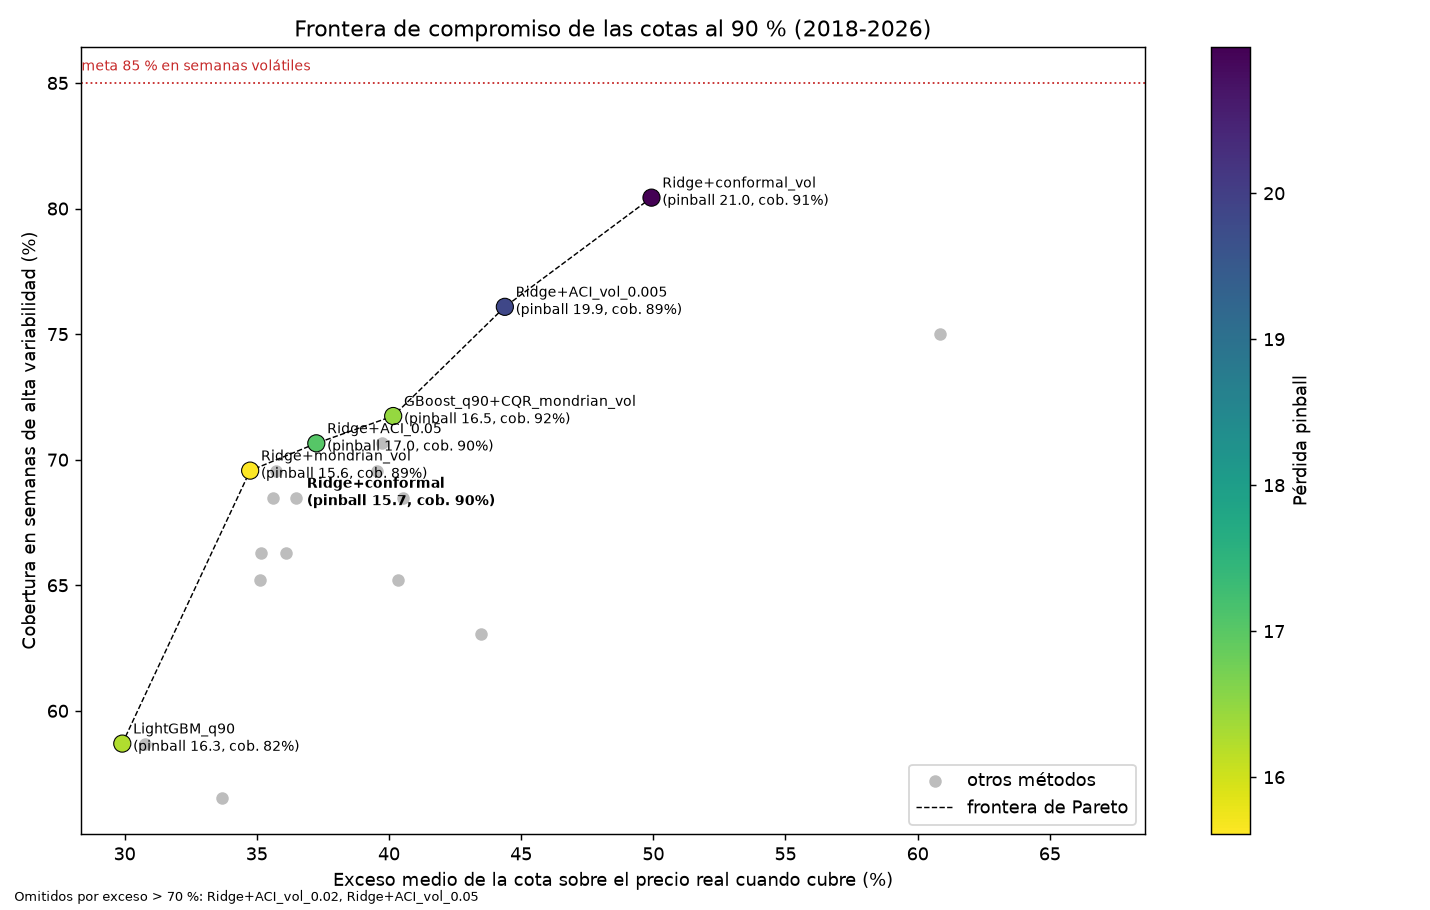
\includegraphics[width=0.85\linewidth]{figuras/E7_frontera_2018-2026.png}
\caption{Compromiso entre el cumplimiento del valor superior en semanas
volátiles y el exceso de garantía, para los métodos evaluados.}
\label{fig:frontera}
\end{figure}

Los métodos más elaborados tampoco cambiaron este panorama. Un modelo
ARIMA, que solo usa la historia del propio precio, apenas mejoró la
referencia simple (0,7\,\%), y las variables construidas en el dominio de
la frecuencia a partir del precio, los aportes y la demanda diarios no
aportaron. La información útil para anticipar la semana siguiente
proviene de la hidrología y de las ofertas, no de la dinámica del propio
precio.

\subsection{El efecto de la información de la semana objetivo}

El único cambio que mejoró con claridad la estimación no fue de método,
sino de información. Cuando la decisión se toma a mitad de semana, ya se
conoce el costo marginal del despacho programado de los primeros días de
la semana objetivo. Incorporarlo redujo el error medio de 54,0 a
39,3\cop{} con dos días conocidos, y a 33,4\cop{} con tres
(Figura~\ref{fig:cmg}). La mejora se mantuvo en los tres periodos
analizados y siguió siendo significativa después de corregir por el
número de alternativas probadas ($p<0{,}001$). Incluso una regla simple,
sin parámetros ajustados, superó al modelo de catorce variables.

\begin{figure}[H]
\centering
\begin{tikzpicture}
\begin{axis}[
  ybar, bar width=22pt, width=0.8\linewidth, height=6cm,
  ymin=0, ymax=78, xmin=0.5, xmax=4.5,
  ylabel={Error medio (COP/kWh)},
  xtick={1,2,3,4},
  xticklabels={Referencia simple,Modelo de 14 variables,
     {+ lunes y martes},{+ lunes a miércoles}},
  xticklabel style={font=\small,text width=2.6cm,align=center},
  nodes near coords, nodes near coords style={font=\scriptsize},
  every node near coord/.append style={/pgf/number format/fixed,
     /pgf/number format/precision=1},
  axis lines*=left, ymajorgrids, grid style={gray!25}]
  \addplot[fill=azul!60,draw=azul] coordinates
    {(1,66.7) (2,54.0) (3,39.3) (4,33.4)};
\end{axis}
\end{tikzpicture}
\caption{Error medio 2018--2026 al incorporar el costo marginal del
despacho programado de los primeros días de la semana objetivo.}
\label{fig:cmg}
\end{figure}

El valor superior también mejoró en las dos direcciones a la vez: su
cumplimiento en las semanas de salto subió de 70\,\% a 76\,\%, y el
exceso medio de garantía bajó de 37\,\% a 23\,\%. Este resultado, sin
embargo, tiene un alcance preciso: ya no es una estimación a una semana
completa, sino a lo que resta de una semana que comenzó. Solo es útil si
la garantía puede fijarse con la semana en curso y si la serie publicada
no se revisa después, dos condiciones que deben confirmarse con XM.

\subsection{Evaluación como clasificación: matrices de confusión}

El error medio resume la exactitud, pero no dice si el modelo anticipa
los movimientos que más importan para la garantía. Para verlo, cada
semana se clasificó según el cambio del precio frente a la semana base:
\emph{baja} (caída de 20\,\% o más), \emph{estable} o \emph{sube}
(aumento de 25\,\% o más). La misma regla se aplicó al cambio que
anticipaba cada modelo. Se compararon los tres modelos que hoy se
registran cada semana: el oficial, de catorce variables; el candidato~1,
que lo promedia con un modelo diario LEAR; y el candidato~2, que añade el
costo marginal programado del lunes y el martes de la semana objetivo.
Los tres se evaluaron en las mismas 456 semanas de 2018--2026 y con los
mismos reentrenamientos (Tabla~\ref{tab:confusion}).

\begin{table}[H]
\centering
\caption{Matrices de confusión del tamaño del cambio semanal,
2018--2026 (número de semanas). Filas: lo que ocurrió; columnas: lo que
anticipó el modelo. La diagonal, en negrita, son los aciertos.}
\label{tab:confusion}
\small
\setlength{\tabcolsep}{3.5pt}
\begin{tabular}{@{}l ccc ccc ccc@{}}
\toprule
 & \multicolumn{3}{c}{\textbf{Oficial}} & \multicolumn{3}{c}{\textbf{Candidato 1}}
 & \multicolumn{3}{c}{\textbf{Candidato 2}} \\
\cmidrule(lr){2-4}\cmidrule(lr){5-7}\cmidrule(l){8-10}
\textbf{Ocurrió} & Baja & Estable & Sube & Baja & Estable & Sube & Baja & Estable & Sube \\
\midrule
Baja (72)     & \textbf{25} & 47 & 0 & \textbf{30} & 42 & 0 & \textbf{43} & 29 & 0 \\
Estable (313) & 11 & \textbf{298} & 4 & 11 & \textbf{299} & 3 & 9 & \textbf{297} & 7 \\
Sube (71)     & 0 & 59 & \textbf{12} & 0 & 59 & \textbf{12} & 1 & 40 & \textbf{30} \\
\midrule
Acierto       & \multicolumn{3}{c}{73,5\,\%} & \multicolumn{3}{c}{74,8\,\%} & \multicolumn{3}{c}{81,1\,\%} \\
Subidas anticipadas & \multicolumn{3}{c}{12 de 71 (17\,\%)} & \multicolumn{3}{c}{12 de 71 (17\,\%)}
 & \multicolumn{3}{c}{30 de 71 (42\,\%)} \\
\bottomrule
\end{tabular}
\end{table}

Las matrices muestran un patrón claro. Ningún modelo confunde una subida
con una caída: casi todos los errores consisten en anticipar estabilidad
cuando el precio se movió con fuerza. El modelo oficial anticipó solo 12
de las 71 subidas de 25\,\% o más, y el candidato~1 no mejora en eso. El
candidato~2 anticipó 30, con una precisión de 81\,\%: de las 37 semanas en
que anticipó una subida, 30 lo fueron. La referencia simple no aparece en
la tabla porque, por construcción, siempre anticipa estabilidad: acierta
el 68,6\,\% de las semanas, que son las estables, y ninguna de las demás.
En el sentido del cambio, sin considerar su tamaño, los aciertos son
73,0\,\%, 74,6\,\% y 79,2\,\%, respectivamente.

La alerta temprana de salto, una regresión logística con su umbral fijado
antes de 2018, es un clasificador binario y se evalúa del mismo modo
(Tabla~\ref{tab:alerta}). Detectó 48 de los 71 saltos (68\,\%), pero solo
el 29\,\% de sus alertas correspondió a un salto. Es útil como aviso para
revisar la garantía, no como señal para ajustarla por sí sola.

\begin{table}[H]
\centering
\caption{Matriz de confusión de la alerta de salto ($P_{s+1}\geq1{,}25\,P_s$),
2018--2026 (número de semanas).}
\label{tab:alerta}
\small
\begin{tabular}{@{}lccc@{}}
\toprule
\textbf{Ocurrió} & \textbf{Sin alerta} & \textbf{Alerta} & \textbf{Total} \\
\midrule
Sin salto & \textbf{272} & 116 & 388 \\
Salto     & 23 & \textbf{48} & 71 \\
\midrule
Total     & 295 & 164 & 459 \\
\bottomrule
\end{tabular}
\end{table}

\subsection{Comparación de los modelos registrados}

La Tabla~\ref{tab:comparacion} resume los tres modelos en la misma
evaluación. El candidato~2 mejora todos los indicadores a la vez: erra
27\,\% menos que el oficial, la diferencia es significativa y su
intervalo está lejos de cero, cumple más el valor superior en las
semanas de salto y exige menos exceso de garantía. El candidato~1 erra
1,4\cop{} menos en todo el periodo, pero esa diferencia deja de ser
significativa al corregir por las alternativas probadas ($p=0{,}52$), y en
las últimas 52 semanas fue peor que el oficial.

\begin{table}[H]
\centering
\caption{Modelos que se registran cada semana: evaluación simulada
2018--2026 en las mismas semanas.}
\label{tab:comparacion}
\small
\begin{tabular}{@{}lccc@{}}
\toprule
\textbf{Indicador} & \textbf{Oficial} & \textbf{Candidato 1} & \textbf{Candidato 2} \\
\midrule
Error medio (COP/kWh) & 54,0 & 52,5 & 39,3 \\
Diferencia frente al oficial & --- & $-1{,}4$ & $-14{,}7$ \\
\quad Intervalo de confianza del 95\,\% & --- & $-2{,}7$ a $-0{,}4$ & $-21{,}2$ a $-10{,}0$ \\
Error medio, últimas 52 semanas & 70,9 & 73,0 & 49,0 \\
Sesgo, últimas 52 semanas & $-33{,}8$ & $-37{,}3$ & $-25{,}9$ \\
Cumplimiento del valor superior & 90,1\,\% & 90,1\,\% & 91,0\,\% \\
Cumplimiento en semanas de salto & 69,6\,\% & 68,5\,\% & 75,0\,\% \\
Exceso medio del valor superior & 37,0\,\% & 35,7\,\% & 28,2\,\% \\
Subidas de 25\,\% o más anticipadas & 17\,\% & 17\,\% & 42\,\% \\
Caídas de 20\,\% o más anticipadas & 35\,\% & 42\,\% & 60\,\% \\
\bottomrule
\end{tabular}
\end{table}

Dos advertencias acotan esta lectura. Primero, la ventaja del candidato~2
proviene de conocer parte de la semana objetivo, así que solo aplica si la
garantía se fija después de que esa semana comienza. Segundo, los tres
comparten un sesgo negativo en el último año: en un periodo de precios al
alza, todos se quedaron cortos. Por eso ninguno reemplaza todavía al
oficial. Desde noviembre de 2026 los tres se registran en paralelo, y la
decisión se tomará con 26 semanas de estimaciones emitidas antes de
conocer el resultado.

\subsection{Cómo cambió el planteamiento}

El trabajo exploratorio dejó cinco aprendizajes que se incorporaron al
problema:

\begin{enumerate}
  \item \textbf{El momento de la decisión importa más que el método.}
        Con la información pública, la semana anterior solo queda
        completa cuando la siguiente ya comenzó; y, si se decide a mitad
        de semana, el despacho programado de esos días reduce el error en
        cerca de 38\,\%. Por eso el momento de decisión pasó a formar
        parte de la pregunta de investigación.
  \item \textbf{El promedio oculta lo importante.} La ventaja frente a la
        referencia simple se concentra en semanas tranquilas. De ahí que
        la pregunta incluya en qué condiciones la estimación deja de ser
        confiable.
  \item \textbf{La confiabilidad tiene un costo.} Cumplir el 90\,\% de
        las semanas implica un exceso medio del 37\,\%. Si ese costo es
        aceptable depende de la regla de la garantía.
  \item \textbf{Las cifras históricas son optimistas.} Al comparar las
        67 alternativas de la etapa principal sobre las mismas semanas,
        la mejor de ellas no supera de forma significativa a la elegida
        ($p=0{,}52$), y en 2025--2026 la
        ventaja frente a la referencia simple no es significativa. Desde
        noviembre de 2026 se lleva un registro de estimaciones emitidas
        antes de conocer el resultado, que será la evidencia independiente.
  \item \textbf{El límite está en la información.} Ningún método más
        complejo superó al lineal, mientras que una sola fuente de
        información nueva ---el despacho programado de la semana
        objetivo--- produjo la mayor mejora del proyecto. El problema es
        de información disponible más que de capacidad de los modelos.
\end{enumerate}

% =====================================================================
\section{Conclusiones y recomendaciones}
% =====================================================================

El problema del caso no es, en sentido estricto, pronosticar el precio de
bolsa, sino fijar una garantía sin saber cuánto puede costar la semana
siguiente ni con qué confiabilidad. Planteado así, el pronóstico es una
de varias respuestas posibles, y su valor depende de la regla de
decisión a la que sirva.

La brecha tiene tres dimensiones ---exactitud, confiabilidad y
oportunidad---, y la tercera no aparecía en la propuesta original: surgió
al medir el rezago real de publicación de los datos. El trabajo
exploratorio mostró, además, que la oportunidad condiciona a las otras
dos: según el día en que se fije la garantía, el error esperado puede
variar de unos 61 a unos 33\cop. Los hechos que
sustentan el problema están documentados con información pública; los
supuestos centrales, en cambio, solo pueden confirmarse con XM.

En consecuencia, se recomienda:

\begin{enumerate}
  \item Confirmar con XM si la necesidad sigue vigente mientras las
        exportaciones estén suspendidas y bajo qué condiciones se
        reanudarían.
  \item Obtener la fórmula vigente de la garantía y el precio que
        interviene en ella, por ser el supuesto con mayor impacto sobre
        la variable de estudio.
  \item Conocer la estimación que se usa hoy y su historial, para
        compararse contra la práctica real y no solo contra una
        referencia simple.
  \item Definir el día y la hora en que debe quedar constituida la
        garantía, y confirmar cuándo se publica el costo marginal del
        despacho programado y si esa serie se revisa después.
  \item Establecer el costo relativo de quedarse corto o excederse, para
        definir el nivel de confiabilidad requerido.
  \item Mantener el registro de estimaciones emitidas como única
        evidencia independiente, y definir con XM cuántas semanas de
        seguimiento serían suficientes.
\end{enumerate}

% =====================================================================
\begin{thebibliography}{9}
% =====================================================================

\bibitem{creg2026}
Comisión de Regulación de Energía y Gas (CREG).
\newblock \emph{Resolución CREG 101~127 de 2026}.
\newblock Bogotá, 2026.

\bibitem{diebold1995}
F.~X. Diebold y R.~S. Mariano.
\newblock Comparing predictive accuracy.
\newblock \emph{Journal of Business \& Economic Statistics}, 13(3):253--263,
  1995.

\bibitem{hoerl1970}
A.~E. Hoerl y R.~W. Kennard.
\newblock Ridge regression: Biased estimation for nonorthogonal problems.
\newblock \emph{Technometrics}, 12(1):55--67, 1970.

\bibitem{lago2021}
J.~Lago, G.~Marcjasz, B.~De~Schutter y R.~Weron.
\newblock Forecasting day-ahead electricity prices: A review of
  state-of-the-art algorithms, best practices and an open-access benchmark.
\newblock \emph{Applied Energy}, 293:116983, 2021.

\bibitem{vovk2005}
V.~Vovk, A.~Gammerman y G.~Shafer.
\newblock \emph{Algorithmic Learning in a Random World}.
\newblock Springer, Nueva York, 2005.

\bibitem{white2000}
H.~White.
\newblock A reality check for data snooping.
\newblock \emph{Econometrica}, 68(5):1097--1126, 2000.

\bibitem{xm}
XM S.A. E.S.P.
\newblock API pública de datos del mercado (Sinergox) y librería
  \texttt{pydataxm}.
\newblock \url{https://github.com/EquipoAnaliticaXM/API_XM}.

\end{thebibliography}

\end{document}
